% Options for packages loaded elsewhere
\PassOptionsToPackage{unicode}{hyperref}
\PassOptionsToPackage{hyphens}{url}
%
\documentclass[
  12pt,
]{article}
\usepackage{amsmath,amssymb}
\usepackage{lmodern}
\usepackage{ifxetex,ifluatex}
\ifnum 0\ifxetex 1\fi\ifluatex 1\fi=0 % if pdftex
  \usepackage[T1]{fontenc}
  \usepackage[utf8]{inputenc}
  \usepackage{textcomp} % provide euro and other symbols
\else % if luatex or xetex
  \usepackage{unicode-math}
  \defaultfontfeatures{Scale=MatchLowercase}
  \defaultfontfeatures[\rmfamily]{Ligatures=TeX,Scale=1}
\fi
% Use upquote if available, for straight quotes in verbatim environments
\IfFileExists{upquote.sty}{\usepackage{upquote}}{}
\IfFileExists{microtype.sty}{% use microtype if available
  \usepackage[]{microtype}
  \UseMicrotypeSet[protrusion]{basicmath} % disable protrusion for tt fonts
}{}
\makeatletter
\@ifundefined{KOMAClassName}{% if non-KOMA class
  \IfFileExists{parskip.sty}{%
    \usepackage{parskip}
  }{% else
    \setlength{\parindent}{0pt}
    \setlength{\parskip}{6pt plus 2pt minus 1pt}}
}{% if KOMA class
  \KOMAoptions{parskip=half}}
\makeatother
\usepackage{xcolor}
\IfFileExists{xurl.sty}{\usepackage{xurl}}{} % add URL line breaks if available
\IfFileExists{bookmark.sty}{\usepackage{bookmark}}{\usepackage{hyperref}}
\hypersetup{
  pdftitle={Supplementary Information},
  hidelinks,
  pdfcreator={LaTeX via pandoc}}
\urlstyle{same} % disable monospaced font for URLs
\usepackage[margin=1in]{geometry}
\usepackage{longtable,booktabs,array}
\usepackage{calc} % for calculating minipage widths
% Correct order of tables after \paragraph or \subparagraph
\usepackage{etoolbox}
\makeatletter
\patchcmd\longtable{\par}{\if@noskipsec\mbox{}\fi\par}{}{}
\makeatother
% Allow footnotes in longtable head/foot
\IfFileExists{footnotehyper.sty}{\usepackage{footnotehyper}}{\usepackage{footnote}}
\makesavenoteenv{longtable}
\usepackage{graphicx}
\makeatletter
\def\maxwidth{\ifdim\Gin@nat@width>\linewidth\linewidth\else\Gin@nat@width\fi}
\def\maxheight{\ifdim\Gin@nat@height>\textheight\textheight\else\Gin@nat@height\fi}
\makeatother
% Scale images if necessary, so that they will not overflow the page
% margins by default, and it is still possible to overwrite the defaults
% using explicit options in \includegraphics[width, height, ...]{}
\setkeys{Gin}{width=\maxwidth,height=\maxheight,keepaspectratio}
% Set default figure placement to htbp
\makeatletter
\def\fps@figure{htbp}
\makeatother
\setlength{\emergencystretch}{3em} % prevent overfull lines
\providecommand{\tightlist}{%
  \setlength{\itemsep}{0pt}\setlength{\parskip}{0pt}}
\setcounter{secnumdepth}{5}
\usepackage{rotating}
\usepackage{setspace}
\usepackage{siunitx}
\usepackage{lscape}
\usepackage{pdfpages}
\newcommand{\beginsupplement}{\setcounter{table}{0}  \renewcommand{\thetable}{A\arabic{table}} \setcounter{figure}{0} \renewcommand{\thefigure}{A\arabic{figure}}}
\usepackage{booktabs}
\usepackage{longtable}
\usepackage{array}
\usepackage{multirow}
\usepackage{wrapfig}
\usepackage{float}
\usepackage{colortbl}
\usepackage{pdflscape}
\usepackage{tabu}
\usepackage{threeparttable}
\usepackage{threeparttablex}
\usepackage[normalem]{ulem}
\usepackage{makecell}
\usepackage{xcolor}
\ifluatex
  \usepackage{selnolig}  % disable illegal ligatures
\fi

\title{Supplementary Information}
\author{}
\date{\vspace{-2.5em}}

\begin{document}
\maketitle

{
\setcounter{tocdepth}{2}
\tableofcontents
}
\pagenumbering{arabic}
\newpage
\doublespacing
\setcounter{table}{0}  \renewcommand{\thetable}{A\arabic{table}} \setcounter{figure}{0} \renewcommand{\thefigure}{A\arabic{figure}}
\newpage

\hypertarget{alternative-specifications-for-regression-discontinuity}{%
\subsection*{Alternative Specifications for Regression Discontinuity}\label{alternative-specifications-for-regression-discontinuity}}
\addcontentsline{toc}{subsection}{Alternative Specifications for Regression Discontinuity}

In the body of this manuscript we present estimated local average treatment effects (LATEs) using a regression discontinuity approach that incorporates both entropy balancing and OLS covariates. Here, we show that our primary results hold when we include only entropy balancing, only OLS covariates, or no adjustment at all.

\begin{figure}[!ht]

{\centering 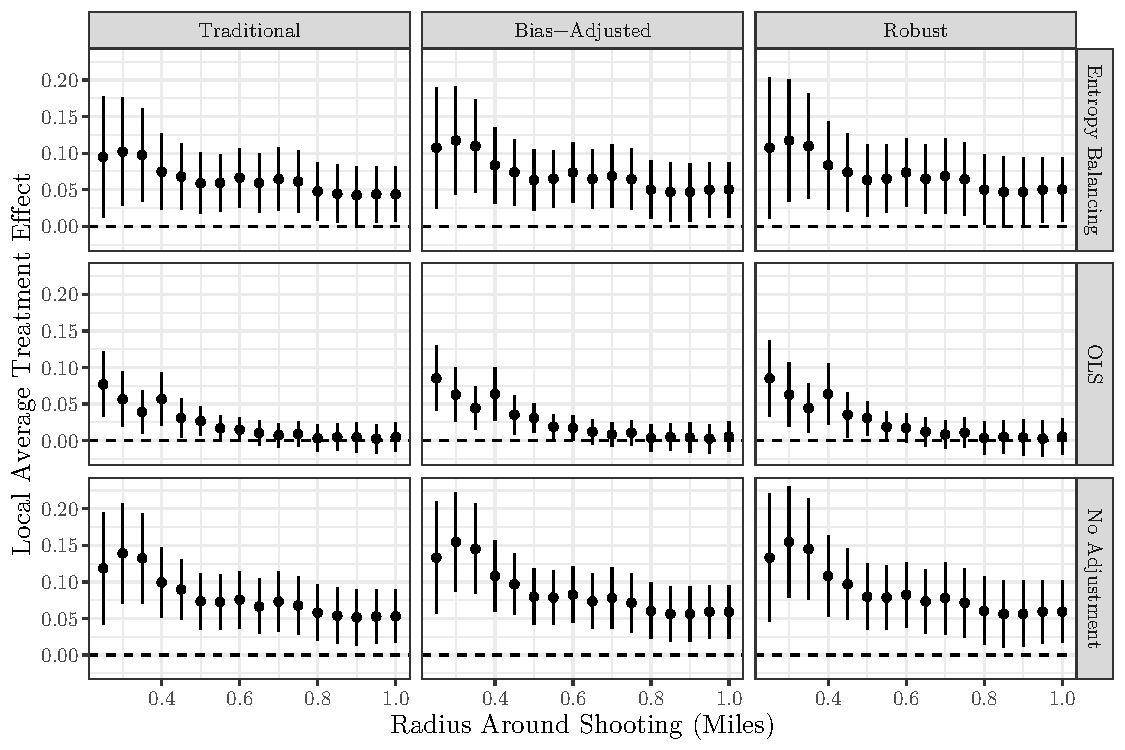
\includegraphics{si_files/figure-latex/alt-proc-1} 

}

\caption{\label{fig:alt-bal}Alternative Approaches for Ensuring Balance Across Cut-Point}\label{fig:alt-proc}
\end{figure}

Figure \ref{fig:alt-bal} makes clear that the overall LATEs we identify in the body of the manuscript are robust to alternative ways of ensuring that observations on either side of the cutpoint closely mirror one another. In fact, the estimated LATEs in the body of the manuscript are in many cases \emph{smaller} than those presented here, indicating that our primary approach is, if anything, conservative.

\hypertarget{robustness-checks-for-primary-rd}{%
\subsection*{Robustness Checks for Primary RD}\label{robustness-checks-for-primary-rd}}
\addcontentsline{toc}{subsection}{Robustness Checks for Primary RD}

Throughout the body of the manuscript, we use a local polynomial of 1, following best practice. In Figure \ref{fig:dif-poly} we show that our primary results for the 0.5-mile threshold are consistent when we use a local polynomial anywhere between 1 and 5. Again, our choice of a local polynomial of 1 appears to be, if anything, a conservative approach.

\begin{figure}[!ht]

{\centering 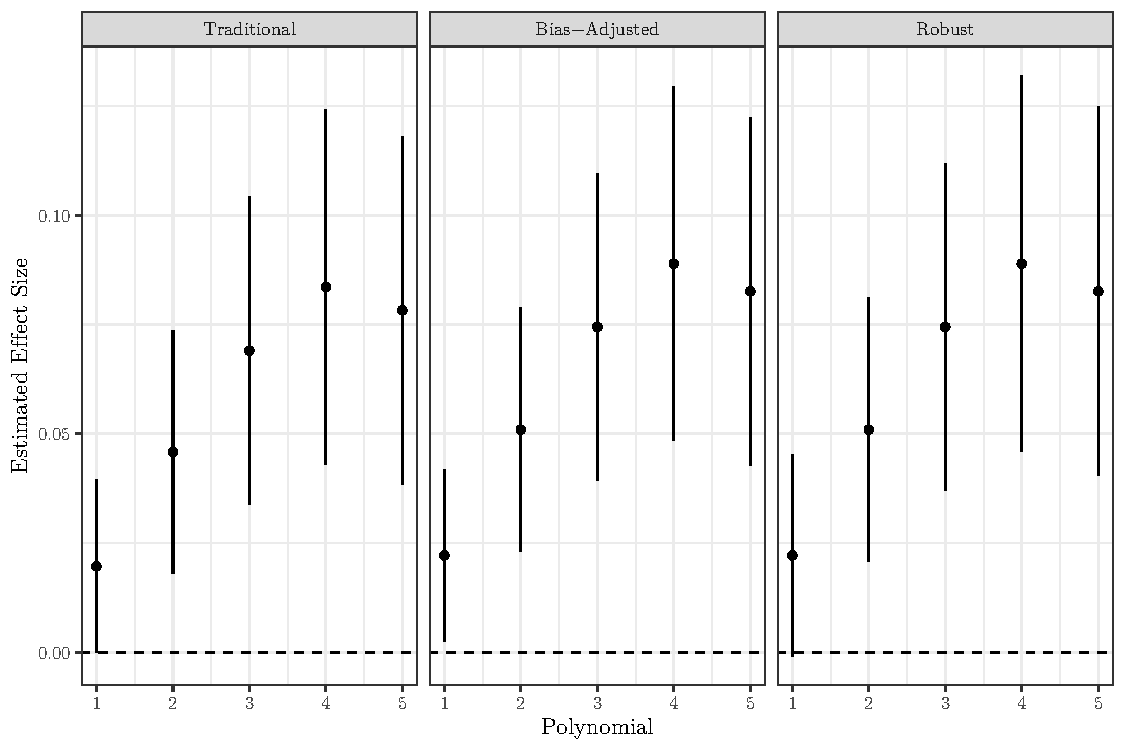
\includegraphics{si_files/figure-latex/diff-poly-1} 

}

\caption{\label{fig:dif-poly}Placebo Alertnate Cut-Points}\label{fig:diff-poly}
\end{figure}

Figure \ref{fig:cutpoint} shows that election day is a meaningful cut-point and that, as expected, other cut-points before and after election day do not map on to meaningul differences in turnout.

\begin{figure}[!ht]

{\centering 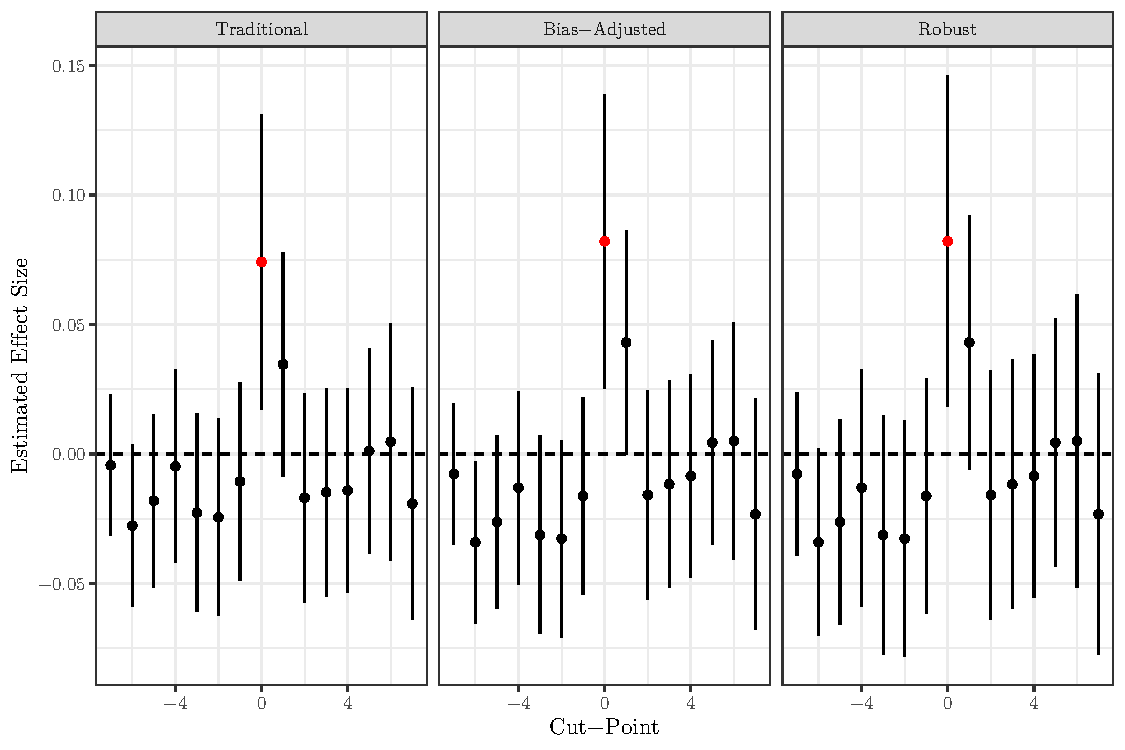
\includegraphics{si_files/figure-latex/placebo-cuts-1} 

}

\caption{\label{fig:cutpoint}Placebo Alertnate Cut-Points}\label{fig:placebo-cuts}
\end{figure}

\end{document}
